\begin{figure}[h!]
\begin{center}
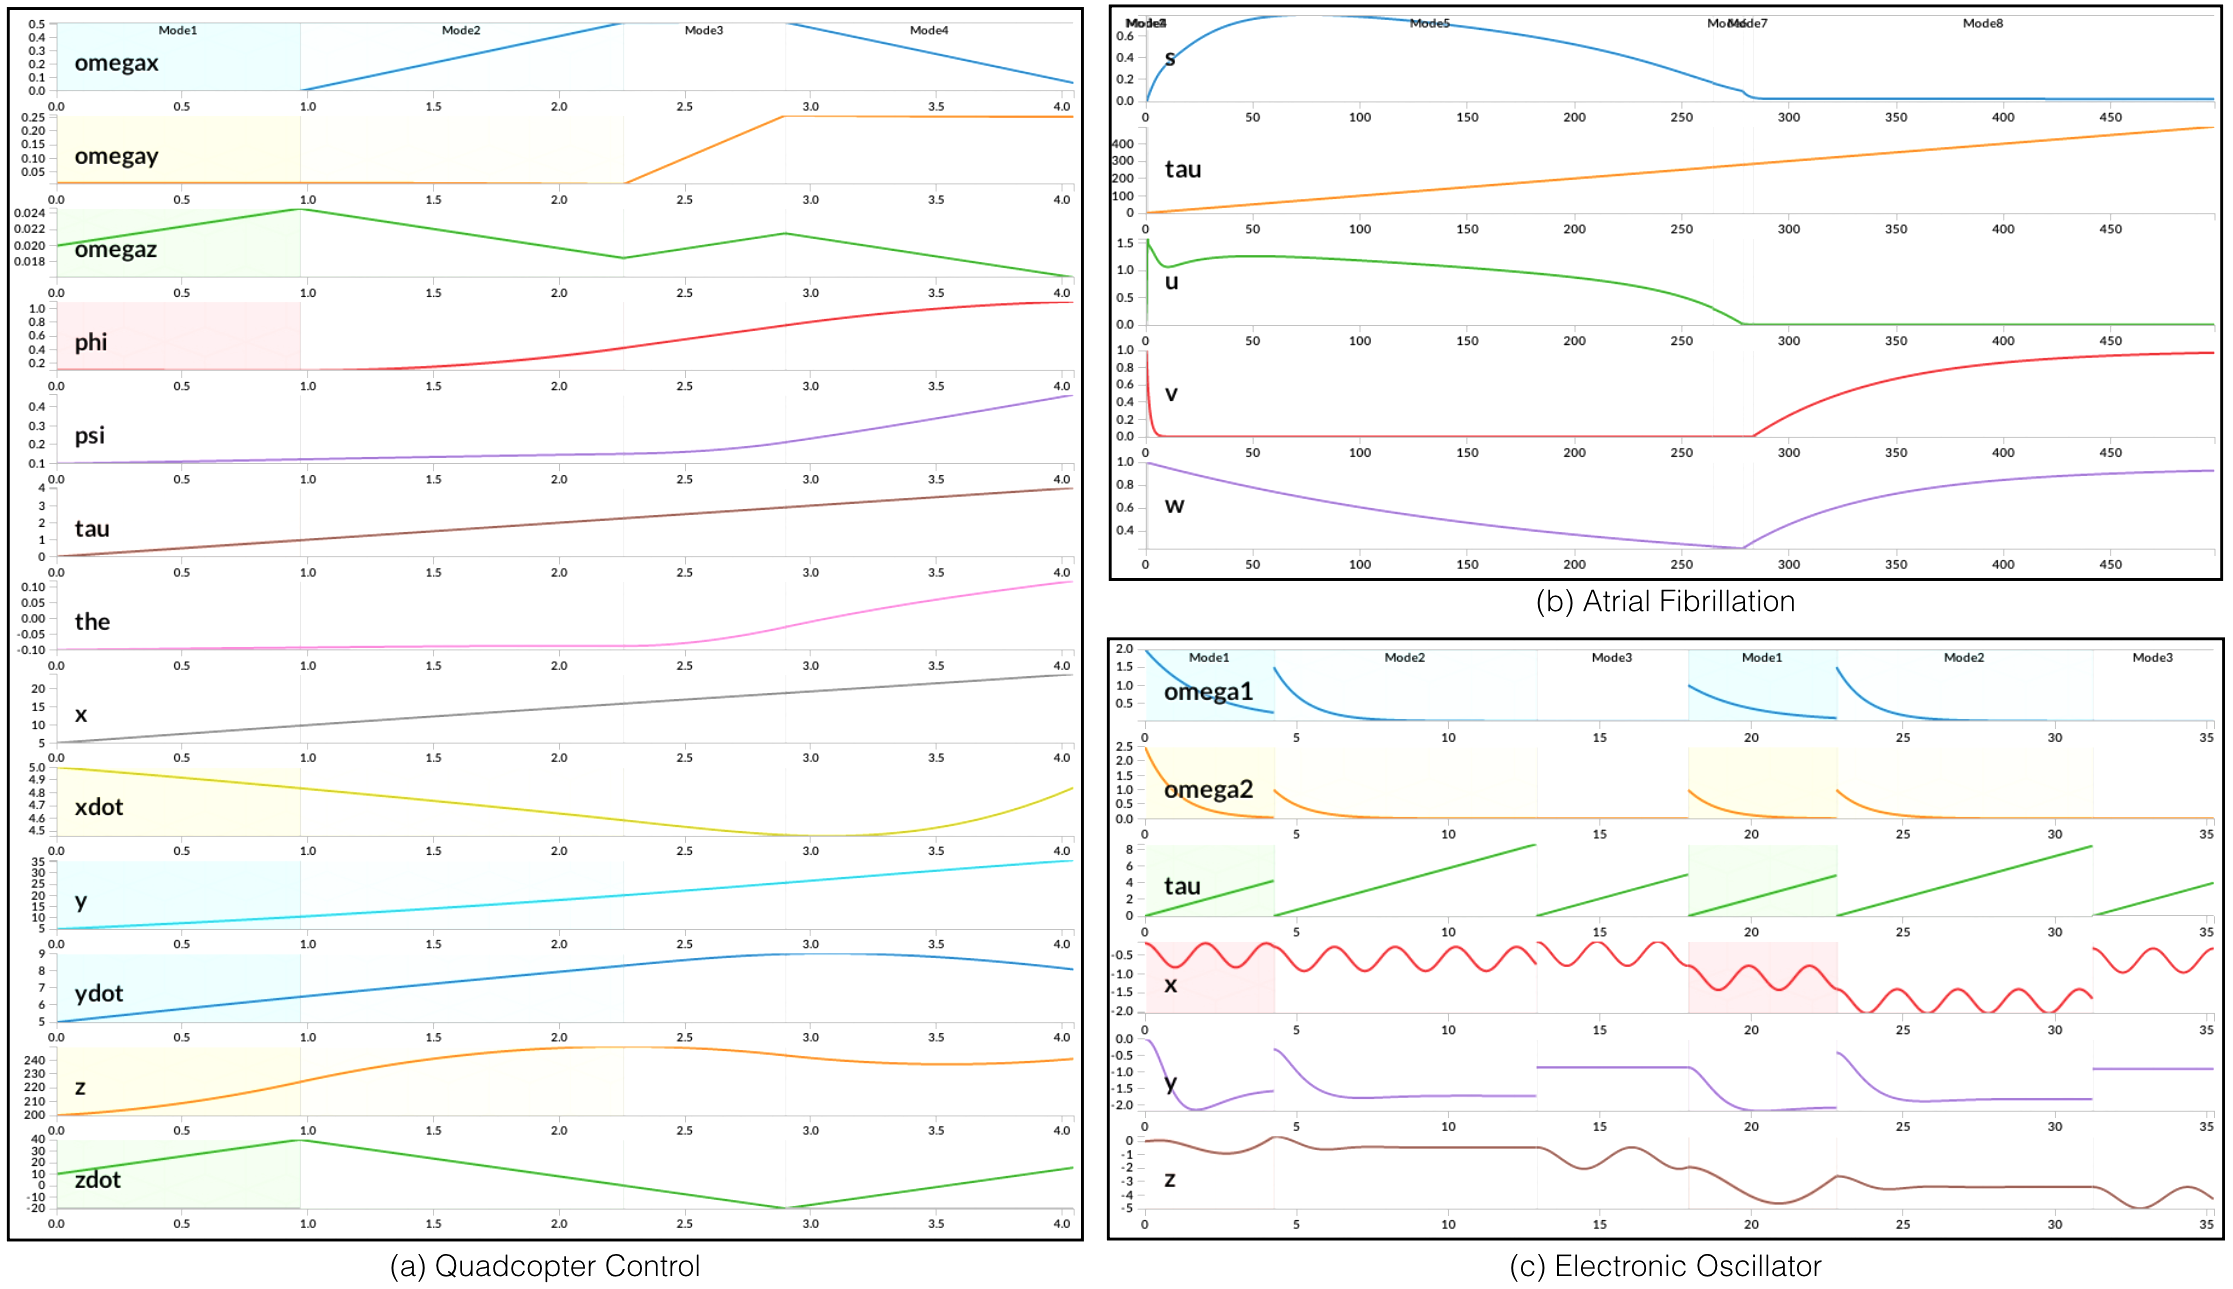
\includegraphics[width=\textwidth]{exp_figure}
\caption{Example trajectories computed for the following models: (a) Quadcopter Control, (b) Atrial Fibrillation, (c) Electronic Oscillator.}\label{fig:exp_figure}
\end{center}
\end{figure}

Our tool {\sf dReal} implements the procedures we studied for solving
SMT formulas with ODEs. It is built on several existing packages,
including {\sf opensmt}~\cite{DBLP:conf/tacas/BruttomessoPST10} for
the general DPLL(T) framework, {\sf
  realpaver}~\cite{DBLP:journals/toms/GranvilliersB06} for ICP, and
{\sf CAPD}~\cite{capd} for computing interval-enclosures of ODEs. The
tool is open-source at~\url{http://dreal.cs.cmu.edu}. All benchmarks
and data shown here are also available on the tool website.

\newcommand{\hmodel}[2]{\href{http://dreal.cs.cmu.edu/#1}{#2}}
{\small
\begin{table}[!th]
  \centering
  \small
  \begin{tabular}{l|r|r|r|r|r|r|r|r}
    \hline
    \hline
    Benchmark    & \#Mode& \#Depth & \#ODEs & \#Vars  & Delta  & Result       & Time(s) & Trace \\
    \hline
    \hline
      AF-GOOD & 4     & 3        & 20     & 53      & 0.001     & S &  0.425    & 793K     \\
       AF-BAD & 4     & 3        & 20     & 53      & 0.001     & U &  0.074    & ---      \\
  AF-TO1-GOOD & 4     & 3        & 24     & 62      & 0.001     & S &  2.750    & 224K     \\
   AF-TO1-BAD & 4     & 3        & 24     & 62      & 0.001     & U &  5.189    & ---     \\
  AF-TO2-GOOD & 4     & 3        & 24     & 62      & 0.005     & S &  3.876    & 553K     \\
   AF-TO2-BAD & 4     & 3        & 24     & 62      & 0.001     & U &  8.857    & ---     \\
 AF-TSO1-TSO2 & 4     & 3        & 24     & 62      & 0.001     & U &  0.027    & ---     \\
       AF8-K7 & 8     & 7        & 40     & 101     & 0.001     & S & 10.478   & 3.8M      \\
      AF8-K23 & 8     & 23       & 40     & 293     & 0.001     & S & 135.29   & 11M      \\
    \hline
    \hline
    EO-K2  & 3     & 2        & 18     & 48      & 0.01    & S & 3.144    & 1.9M      \\
    EO-K11 & 3     & 11       & 99     & 174     & 0.01    & U & 0.969    & ---       \\
    \hline
    \hline
    QUAD-K1  & 2   & 1          & 34     & 89      & 0.01      & S & 2.386 &  10M \\
    QUAD-K2  & 2   & 2          & 34     & 125     & 0.01      & S & 4.971 &  13M \\
    QUAD-K3  & 4   & 3          & 68     & 161     & 0.01      & S & 13.755 & 42M \\
    QUAD-K3U & 4   & 3          & 68     & 161     & 0.01      & U & 2.846 & --- \\
    \hline
    \hline
    CT       & 2   & 2         & 10      & 41      & 0.005     & S & 345.84 & 3.1M\\
    CT       & 2   & 2         & 10      & 41      & 0.002     & S & 362.84 & 3.1M\\
    \hline
    \hline
    BB-K10 & 2     & 10       & 22     & 66      & 0.01        & S & 8.057     & 123K  \\
    BB-K20 & 2     & 20       & 42     & 126     & 0.01        & S & 39.196    & 171K  \\
    \hline
    \hline
  \end{tabular}
  \caption{\small
    \#Mode = Number of modes in the hybrid system,
    \#Depth = Unrolling depth,
    \#ODEs = Number of ODEs in the unrolled formula,
    \#Vars = Number of variables in the unrolled formula,
    Result = Bounded Model Checking Result (delta-SAT/UNSAT)
    Time = CPU time (s),
    Trace = Size of the ODE trajectory,
    AF = Atrial Filbrillation,
    EO = Electronic Oscillator,
    QUAD = Quadcopter Control,
    CT = Cancer Treatment,
    BB = Bouncing Ball with Drag.
    % TIMES = Solving time in seconds, TO = Timeout (30min), PC = Proof
    % Checked, #PA = Number of proved axioms, #SP = Number of subproblems
    % generated by proof checking, TIMEPC = Proof-checking time in seconds, #D =
    % Number of iteration depth required in proof checking
}\label{tbl:exp}
\end{table}
}
%%% Local Variables:
%%% mode: latex
%%% TeX-master: "delta_reachability.tex"
%%% End:
